\documentclass[tikz,border=4pt]{standalone}
\usepackage[T1]{fontenc}
\usepackage{lmodern}
\usetikzlibrary{arrows.meta,calc,positioning}
\ifdefined\darkmode
  \definecolor{paper}{HTML}{17191B}\definecolor{ink}{HTML}{D7D7D3}
  \definecolor{muted}{HTML}{969A9C}\definecolor{accent}{HTML}{7F9EAE}
  \definecolor{solar}{HTML}{C4A56C}\definecolor{line}{HTML}{3B4043}
  \definecolor{panel}{HTML}{202326}\definecolor{penumbrafill}{HTML}{403B32}
  \definecolor{umbrafill}{HTML}{334852}
\else
  \definecolor{paper}{HTML}{F5F5F2}\definecolor{ink}{HTML}{202326}
  \definecolor{muted}{HTML}{666B70}\definecolor{accent}{HTML}{315F78}
  \definecolor{solar}{HTML}{8A6428}\definecolor{line}{HTML}{CFD2D2}
  \definecolor{panel}{HTML}{ECEEEC}\definecolor{penumbrafill}{HTML}{E5DDCE}
  \definecolor{umbrafill}{HTML}{B8CBD5}
\fi
\begin{document}\sffamily
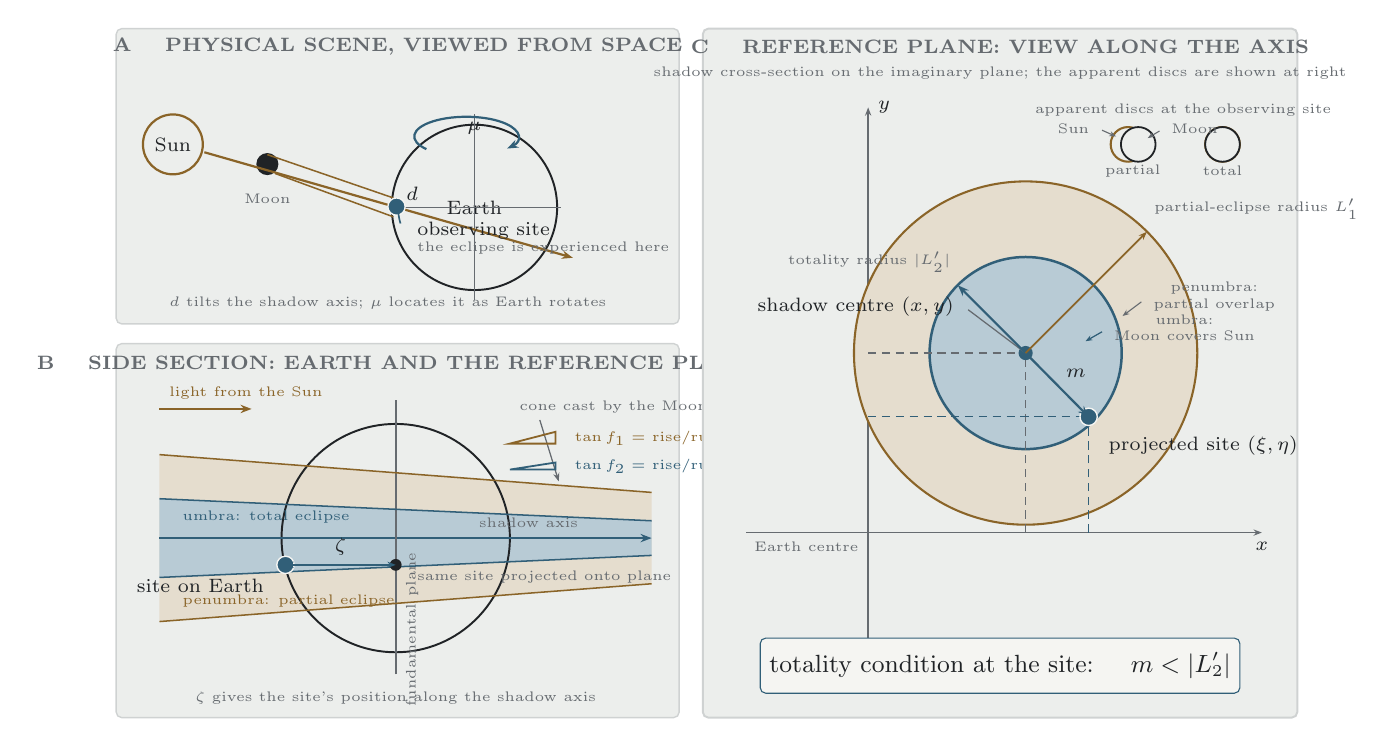
\begin{tikzpicture}[x=1cm,y=1cm,
  title/.style={text=muted,font=\bfseries\scriptsize},
  label/.style={text=ink,font=\scriptsize},
  note/.style={text=muted,font=\tiny,align=center},
  axis/.style={draw=accent,line width=.8pt,-{Stealth[length=4pt]}},
  guide/.style={draw=muted,densely dashed,line width=.45pt},
  dim/.style={draw=accent,line width=.65pt,{Stealth[length=3pt]}-{Stealth[length=3pt]}},
  frame/.style={draw=line,fill=panel,rounded corners=2pt,line width=.5pt}
]
% Physical-space inset
\draw[frame] (0,5.0) rectangle (7.15,8.75);
\node[title] at (3.575,8.52) {A \quad PHYSICAL SCENE, VIEWED FROM SPACE};
\draw[solar,line width=.8pt] (.72,7.28) circle (.38);
\node[label] at (.72,7.28) {Sun};
\fill[ink] (1.92,7.03) circle (.14);
\node[note,below=2pt] at (1.92,6.84) {Moon};
\draw[ink,line width=.7pt] (4.55,6.48) circle (1.05);
\node[label] at (4.55,6.48) {Earth};
\draw[muted,line width=.45pt] (4.55,5.3)--(4.55,7.66);
\draw[muted,line width=.45pt] (3.45,6.48)--(5.65,6.48);
\draw[solar,line width=.8pt,-{Stealth[length=4pt]}] (1.12,7.18)--(5.8,5.84);
\draw[solar,line width=.55pt] (2.02,6.91)--(3.52,6.36);
\draw[solar,line width=.55pt] (1.92,7.15)--(3.52,6.60);
\fill[accent,draw=paper,line width=.5pt] (3.56,6.49) circle (.11);
\node[label,anchor=west] at (3.7,6.18) {observing site};
\node[note,anchor=west] at (3.7,5.96) {the eclipse is experienced here};
\draw[accent,line width=.6pt] (3.58,6.48) arc (180:197:.7);
\node[label] at (3.76,6.65) {$d$};
\draw[axis] (3.94,7.22) arc (220:-38:.66 and .25);
\node[label] at (4.55,7.48) {$\mu$};
\node[note] at (3.45,5.27) {$d$ tilts the shadow axis; $\mu$ locates it as Earth rotates};

% Side-section inset
\draw[frame] (0,0) rectangle (7.15,4.75);
\node[title] at (3.575,4.51) {B \quad SIDE SECTION: EARTH AND THE REFERENCE PLANE};
% Explicit palette fills remain distinguishable in both system themes.
\fill[penumbrafill] (.55,1.22)--(6.8,1.70)--(6.8,2.86)--(.55,3.34)--cycle;
\fill[umbrafill] (.55,1.78)--(6.8,2.06)--(6.8,2.50)--(.55,2.78)--cycle;
\draw[ink,line width=.7pt] (3.55,2.28) circle (1.45);
\draw[accent,line width=.75pt,-{Stealth[length=4pt]}] (.55,2.28)--(6.8,2.28)
  node[near end,above,note] {shadow axis};
\draw[muted,line width=.8pt] (3.55,.55)--(3.55,4.04);
\node[note,rotate=90] at (3.76,1.12) {fundamental plane};
\draw[solar,line width=.55pt] (.55,1.22)--(6.8,1.7) (.55,3.34)--(6.8,2.86);
\draw[accent,line width=.55pt] (.55,1.78)--(6.8,2.06) (.55,2.78)--(6.8,2.50);
\node[text=solar,anchor=west,font=\tiny] at (.72,1.48) {penumbra: partial eclipse};
\node[text=accent,anchor=west,font=\tiny] at (.72,2.55) {umbra: total eclipse};
\draw[solar,line width=.8pt,-{Stealth[length=4pt]}] (.55,3.92)--(1.72,3.92);
\node[text=solar,anchor=west,font=\tiny] at (.55,4.12) {light from the Sun};
\node[note,anchor=west] at (5.00,3.95) {cone cast by the Moon};
\draw[muted,line width=.45pt,-{Stealth[length=3pt]}] (5.38,3.78)--(5.62,3.00);
% Small rise/run constructions make the cone-slope parameters literal.
\draw[solar,line width=.65pt] (5.00,3.48)--(5.58,3.48)--(5.58,3.63)--cycle;
\node[text=solar,anchor=west,font=\tiny] at (5.70,3.55) {$\tan f_1=$ rise/run};
\draw[accent,line width=.65pt] (5.00,3.15)--(5.58,3.15)--(5.58,3.24)--cycle;
\node[text=accent,anchor=west,font=\tiny] at (5.70,3.19) {$\tan f_2=$ rise/run};
\fill[accent,draw=paper,line width=.5pt] (2.15,1.94) circle (.11);
\node[label,anchor=east] at (2.0,1.68) {site on Earth};
\fill[ink] (3.55,1.94) circle (.075);
\draw[dim] (2.15,1.94)--(3.55,1.94);
\node[label,above] at (2.85,1.94) {$\zeta$};
\node[note,anchor=west] at (3.7,1.78) {same site projected onto plane};
\node[note] at (3.55,.25) {$\zeta$ gives the site's position along the shadow axis};

% Face-on calculation panel
\draw[frame,line width=.7pt] (7.45,0) rectangle (15.0,8.75);
\node[title] at (11.225,8.52) {C \quad REFERENCE PLANE: VIEW ALONG THE AXIS};
\node[note] at (11.225,8.18) {shadow cross-section on the imaginary plane; the apparent discs are shown at right};
\draw[muted,line width=.5pt,-{Stealth[length=3pt]}] (8.0,2.35)--(14.55,2.35) node[below,label] {$x$};
\draw[muted,line width=.5pt,-{Stealth[length=3pt]}] (9.55,.72)--(9.55,7.75) node[right,label] {$y$};
\node[note,below left] at (9.55,2.35) {Earth centre};
\coordinate (shadow) at (11.55,4.63);
\coordinate (site) at (12.35,3.82);
\fill[penumbrafill] (shadow) circle (2.18);
\fill[umbrafill] (shadow) circle (1.22);
\draw[solar,line width=.75pt] (shadow) circle (2.18);
\draw[accent,line width=.9pt] (shadow) circle (1.22);
\draw[guide] (9.55,4.63)--(shadow) (11.55,2.35)--(shadow);
\draw[guide,accent] (9.55,3.82)--(site) (12.35,2.35)--(site);
\fill[accent] (shadow) circle (.09);
\fill[accent,draw=paper,line width=.5pt] (site) circle (.11);
\draw[axis] (shadow)--(site);
\draw[muted,line width=.45pt] (shadow)--(10.82,5.18);
\node[label,anchor=east] at (10.76,5.22) {shadow centre $(x,y)$};
\node[label,anchor=north west] at (12.48,3.70) {projected site $(\xi,\eta)$};
\node[label,anchor=south west] at (11.94,4.20) {$m$};
\draw[axis] (shadow)--++(-.86,.86);
\node[note,anchor=south east] at (10.72,5.53) {totality radius $|L'_2|$};
\draw[solar,line width=.65pt,-{Stealth[length=3pt]}] (shadow)--++(1.54,1.54);
\node[note,anchor=south west] at (13.06,6.2) {partial-eclipse radius $L'_1$};
% Apparent-disc legend: these are the Sun and Moon as the observer sees them.
\node[note] at (13.55,7.72) {apparent discs at the observing site};
\draw[solar,line width=.75pt] (12.85,7.28) circle (.22);
\fill[panel,draw=ink,line width=.65pt] (12.98,7.28) circle (.22);
\node[note] at (12.91,6.94) {partial};
\draw[solar,line width=.75pt] (14.05,7.28) circle (.22);
\fill[panel,draw=ink,line width=.65pt] (14.05,7.28) circle (.22);
\node[note] at (14.05,6.94) {total};
\node[note,anchor=east] at (12.48,7.48) {Sun};
\draw[muted,line width=.4pt,-{Stealth[length=2.5pt]}] (12.52,7.46)--(12.70,7.38);
\node[note,anchor=west] at (13.28,7.48) {Moon};
\draw[muted,line width=.4pt,-{Stealth[length=2.5pt]}] (13.25,7.45)--(13.10,7.36);
\node[note,anchor=west] at (13.05,5.35) {penumbra:\\partial overlap};
\draw[muted,line width=.4pt,-{Stealth[length=2.5pt]}] (13.02,5.28)--(12.78,5.10);
\node[note,anchor=west] at (12.55,4.95) {umbra:\\Moon covers Sun};
\draw[accent,line width=.45pt,-{Stealth[length=2.5pt]}] (12.52,4.90)--(12.31,4.78);
\node[draw=accent,rounded corners=2pt,fill=paper,text=ink,font=\small,
  minimum width=5.3cm,minimum height=.7cm] at (11.225,.66)
  {totality condition at the site: \quad $m<|L'_2|$};
\end{tikzpicture}
\end{document}
